
\chapter{Requirements Overview}
\label{cha:require}

This chapter gives a complete overview specification of the
requirements for \Pyb.

For a general view of \textit{existing} bibliographical and related
applications see \textit{supra} \ref{sec:introevo}.  The existing
interfaces are detailed below at \ref{sec:reqinterface} insofar as
they remain relevant.  General usage considerations can be found also
in Part II. -- A summary statement of purpose is given at the beginning
of chapter~\ref{cha:intro}.


General information can also be found in the \textit{User's Guide}. 


\section{Goals and Purposes}
\label{sec:reqgoals}

\cbstart

Many people, and academics in particular collect a set of references
or citations.  Historically, this collection may have been contained
on a set of index cards.  However, for some time now, programs have
been used to help with the tedious aspects of the work, in particular
if the number of references has grown into hundred or thousands.

Bibliographic database managers or \textit{reference managers} are a
specialized type of a database manager designed for the handling of
bibliographic references. They are also known as personal information
systems, bibliographic reference managers, or personal bibliographic
software. These systems help with essential research or publishing
tasks:\footnote {this discussion is taken from \cite{sat:hsu01} and
  \cite{bib:uwa00}} 

\begin{itemize*}
\item Building a database of references to journal articles, books, and
  other research publications, using both manual and electronic
  input methods 
\item  Searching the created database by author, subject, journal name,
  and other criteria 
%\item  Generating a list of selected references from
%  the database in a specified format for various purposes
% \item Maintenance of a database of references. 
% \item Downloading references 
\item Using the database to link references in word processed
  documents. 
\item Generate the bibliography in the correct style for publication. 
\item Output to separate file for interchange or printing. 
\end{itemize*}


Such a database, once established, might be put to many uses, some
examples (with modifications taken frm from \citep{sat:hsu01}) follow:
\begin{itemize*}
\item Create course reserve lists and reading lists for students
\item Maintain faculty publication lists 
\item Catalog special collections 
\item Keep track of reprint collections 
\item Maintain bibliographies of references in research areas of
  personal interest  
\item Prepare instantaneous formatted in-text citations and
  bibliographies during manuscript preparation  
\item Create and maintain a reference database shared among a group of
  resources across a network  
\item Publish a web-based bibliography 

\end{itemize*}

Reference manager software has been around for a number of years, but
lately has assumed a larger role, and faces new challanges owing to
several recent advances, as follows:

\begin{itemize*}
\item Tighter integration with word processors. --   These features enable
  you to insert references from your bibliographic database while you
  type. 
\item Conversely, the flow of information from the Editor\slash Word
  processor comes into focus, with ideas such as imbedding full
  bibliographic records into documents and automatic tracking of
  citations. 
\item Z39.50 Search and Retrieval Protocol -- Many library catalogues
  are accessible over the internet via this protocol.  This means that
  the user can search the catalogues of any accessible library, and
  download references directly into his personal bibliographic
  database.
\item This exposes the user to a mixture of descriptions that are
  often more detailed and use more sophisticated methods of
  description than what he is used to.
\item The Web --  PBM software can link directly from a URL in a citation
  to the supporting site and also open a locally stored  document.  
\item In addition the web browser has become the universal virtual
  terminal, allowing access from every place in the world.   Therefore
  many wish to publish their bibliographies on the web, and perhaps
  even more.
\item This development has led to a re-appraisal of many received ideas
  and rules, leading to a more fully understanding of the issues
\item The gap that, e.g., has separated library and archival theory
  and practice, is slowly narrowing.  Thus it becomes conceivable to
  intergrate more types of resources, i.e., the unique resources the
  office and archive deals with, or the products of project work, that
  hithereto received only haphazard attention.  
\end{itemize*}

\cbend 

\section{Program Audience and Context}
\label{sec:reqcont}

The intended main user of this program is the academic scholar\slash
writer, who needs a tool to maintain his growing set of references and
to access his own and other databases and document repositories.  The
\textit{workflow 2} captures the essence of these transactions with the
system, as the purpose is usually to author own documents.

In work group settings the inquiry-only type of operation
\textit{(workflow 1)} will supposedly become more important; consider
students using a \textit{bibliography server}. -- Note that, in any
case, searching and browsing are the fundamental interactions with the
system and have the greatest usability impact.

The degree of administrative\slash programming and cataloguing\slash
organising work, as detailed in \textit{workflow 3} will vary greatly.
Major factors are:
\begin{enumerate*}
\item Individual vs.\ collaborative use.
\item The degree of detail needed, e.g., maintaing a database for long
  term use requires a greater level of detail than short time, project
  type work.
\item Standard bibliogrpahical description vs.\ special needs, such as
  recording of archival sources, which may involve unique data
  acquisition requirements, such as complex case histories.
\item Standard reference lists \textit{� la} Bib\TeX\ vs.\ complicated
  output processing, e.g., a web based classified, annotated
  bibliography.
\end{enumerate*}

\begin{dnote}  
\item The above points should be explained in User's Guide chapters
  \ref{UG.cha:rgintro} and \ref{UG.cha:rgprep}.
\end{dnote}

The  context is further defined by the interfaces to:
\begin{enumerate*}
\item Document repositories, local and remote.
\item Other databases and sources of information -- mainly Query and
  Import interface.
\item Document preparation tools -- to be defined, except for Bib\TeX\ 
  compatibility.
\item Output processors -- XSLT should unify this.
\end{enumerate*}

Typical workflows are explained below.  In the last column, references
are given to the \textit{Use cases} in section \ref{sec:requsecase}.
In general the workflows can be subdivided into the following stages
and tasks:
\label{sec:workflow1}

\cbstart

\begin{table}[htbp]\sffamily\small
  \begin{tabular}[t]{|l|p{10cm}|p{3cm}|}
\hline \textbf{Stage}& \textbf{Description}&\textbf{Related}\\ \hline
\textbf{1}& Choose a database, \textit{if necessary}&
\textit{\rmfamily 011}\\
\textbf{2}& Do a \textit{Known-Item-Search}, e.g., with an author\slash
title pair, \textit{or even}& \textit{\rmfamily 001}\\
\textbf{3}& Formulate an \textit{expert query}, this requires some
   acquaintance with the data base, \textit{or}& \textit{\rmfamily 003}\\
\textbf{4}& \textit{Browse an Index}, if you are looking for things you
   don't know beforehand (or might have forgotten), e.g., in a Journals
   Index,  \textit{or}&\textit{\rmfamily 010}\\
\textbf{5}& Follow a cross-reference, e.g., by looking at the works of an
   author, or papers which cite another.&\\
\textbf{6}&  \textit{Look over the results.} Examine individual
records. &\\
\textbf{7}& Based on the results, variate or make more precise the search
   question.&\textit{\rmfamily 002}\\
\textbf{8}&  Mark items to set them aside for further examination or
   processing.&\textit{\rmfamily 007, 008}\\
\textbf{9}& Add a note  to an item.&\textit{\rmfamily 005, 008}\\
\textbf{10}& Output all or any of the items, in various formats, to another
   file, to the clipboard for inclusion in another document
   (using \textit{Drag-and-drop}), to the printer. &\textit{\rmfamily 006}\\
\hline
  \end{tabular}
  \label{tab:workflow1}
\end{table}

\cbend

\subsection{Scenario: Write a Paper}
\label{sec:workflow2}

Within the following scenario, you will find yourself searching and
browsing (as above in \ref{sec:search-browse}) many times; now these
\textit{Use Cases} are imbedded in more complex processes. So, e.g.,
stages 6 and 7 below consist not only of searching and browsing
activities, but integrate them with the writing process: an item is
not only found, but it's citation is included in the document in
preparation, it is placed on or taken from a work list, a reference is
linked back to the cited item etc.

\begin{table}[htbp]\sffamily\small
  \begin{tabular}[t]{|l|p{10cm}|}
\hline \textbf{Stage}& \textbf{Description}\\ \hline
&\textbf{Collect Information}\\
\textbf{1}& Maintain a reading list.\\
\textbf{2}& Acquire information from databases.\\
\textbf{3}& Acquire information from other sources.\\
\textbf{4}& Add notes and quotes.\\
& \textbf{Write}\\
\textbf{5}& Maintain a work plan.\\
\textbf{6}& Find items, notes, quotes, etc.\\
\textbf{7}& Insert and mark-up references and quotes.\\
\textbf{8}& Audit work done. (Check cited works, etc.)\\
\textbf{9}& Process references for output formatting.\\
\hline
  \end{tabular}
  \label{tab:workflow1}
\end{table}

\subsection{Scenario: Maintain a Bibliography}
\label{sec:workflow3}

The linking process that lies at the core of \Pyb's support of the
writing process is applied in the next, most demanding situation to
documents of various kinds that are \textit{given} and
\textit{augmented} for better analysis and access.
% Now consider another  situation, where you want to build and maintain
% a website devoted to your favourite writer, A.U.~Thor.   Of course,
% you will want to make maximum use of your computer and derive the
% web presentation from the database. \dots

% A special need is to keep track of things coming in.
% Take reviews, which must be somehow related to the subject work \dots


\begin{table}[htbp]\sffamily\small
  \begin{tabular}[t]{|l|p{10cm}|}
\hline \textbf{Stage}& \textbf{Description}\\ \hline
\textbf{1}& Organise work.\\
\textbf{2}& Add and import records.\\
\textbf{3}& Check, edit and merge records.\\
\textbf{4}& Add documents.\\
\textbf{5}& Describe (mostly) archival items and collections.\\
\textbf{6}& Maintain authority data. \\
\textbf{7}& Add and edit access points.\\
\textbf{8}& Add annotations, other texts.\\
\textbf{9}& Process output.\\
\textbf{10}& Export data for backup, integration.\\
\hline
  \end{tabular}
  \label{tab:workflow1}
\end{table}



\section{Interfaces}
\label{sec:reqinterface}


\subsection{Actors and Activities}
\label{sec:ov-actors}

\begin{table}[hbp]
  \centering
  \begin{tabular}[t]{|l|p{.8\textwidth}|}
\hline
\textbf{\sffamily Actors}& \textbf{\sffamily Description}\\
\hline
\textbf{\sffamily User}& assumes different roles:
\begin{itemize}
\item \textit{searches} internal and external databases
\item \textit{adds} references and notes
\item \textit{formats} reference lists and bibliographies
\item \textit{accesses} external documents 
\item \textit{administrates} Pybliographer itself.
\end{itemize}\\

\hline
  \end{tabular}
  \caption{Actors}
  \label{tab:actors}
\end{table}


\subsection{External Interfaces}
\label{sec:reqextint}


\subsection{Internal Interfaces}
\label{sec:reqintint}



% Allgemeines
% Ist-Aufnahme und Ist-Analyse

% 6. 1. Grobe Systembeschreibung
% 6. 2. Organisatorische Einbettung
% 6. 3. Nutzung
% 6. 4. Kritikalit�t des Systems
% 6. 5. Externe Schnittstellen
% 6. 6. Beschreibung der Funktionalit�t
% 6. 7. Qualit�tsforderungen

\section{Program Features}
\label{sec:reqfeat}

The program offers the standard features of similar programs, as shown
in Appendix \ref{cha:commfeat}. 

\begin{table}[htbp]
  \centering
  \begin{tabular}[t]{|c|p{.6\textwidth}|l|l|}
\hline
Ref.& Description& Related&See also\\
\hline
R010& Entering, merging records& 9004&\\
R020& Searching records& 9001&\\
R030& External search, importing data& 9002&\\
R040& Formatting bibliographies and citations. & 9005&\\
R050& Efficient database&&\\
R060& Adequate, extensible database schema& 9006&\\
R070& Adequate classification&&\\
R080& Annotations of various types&&\\
R090& Multiple languages and scripts&&\\
 \hline
  \end{tabular}
  \caption{Mandatory Features}
  \label{tab:reqmand}
\end{table}

\subparagraph{Optional functions}

\begin{itemize*}
\item Connection with word processors and Emacsen.
\item Web interface
\item Work group support
\item Archival support
\item Spell checking and other input enhancements
\end{itemize*}


\subparagraph{Excluded functions}

\begin{itemize*}
\item Library loan and acquisition functions.
\item Repository and collection management. 
\item Sophisticated output -- only BibTeX level

\end{itemize*}


%\section{Use Cases}


\begin{figure}[htbp]
  \centering
  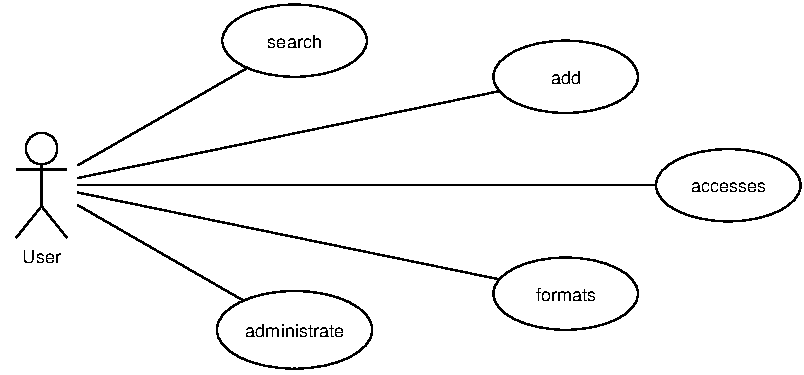
\includegraphics[width=.8\textwidth]{pics/ov-uc-001}
  \caption{Use case diagram (overview)}
  \label{fig:ov-usecase}
\end{figure}

\textit{Note:} Perhaps it is better to use the describe -- organise --
refer structure from \ref{sec:summrequ} supra?

\newenvironment{usecaselist}{%
\section{Usecases}
\label{sec:requsecase}
\tablehead{\firsthline}
{\tabletail{\lasthline}}
\begin{center}\begin{supertabular}{|l|p{11cm}|p{3cm}|}}
  {\end{supertabular}\end{center}}

\newcommand{\ucitem}[4]{#1& \textbf{#2} #3& #4\\}


% \begin{table}[htbp]
%   \centering
%   \begin{tabular}[t]{|l|p{.8\textwidth}|}
% \hline
% \textbf{\sffamily Use case} & \textbf{\sffamily Description}\\
% \hline

\begin{usecaselist}
\input{tx-use.lst}  
\end{usecaselist}





% \hline
%   \end{tabular}
%   \caption{Activities (use cases)}
%   \label{tab:ov-usecase}
% \end{table}

\newpage

\cbstart 


\section{Requirements Directory}
\label{sec:reqrequ}

The following table directs you to the detailed lists of functional
requirements that are distributed over this document. 

\begin{enumerate*}
\item Generalities
  \begin{enumerate*}
  \item Packageing and Installation
  \item Documentation
  \item Authorisation and Protection
  \end{enumerate*}
\item Bibliographical description
  \begin{enumerate*}
  \item Generalities
  \end{enumerate*}
\item Subject description and access 
  \begin{enumerate*}
  \item Generalities
  \item Persons
  \item Subject Headings 
  \item Classifications
  \item Coded lists and Classifiers
  \item Keywords, etc.
  \item Full text search
  \end{enumerate*}
\item User Interface, Input, and Import
  \begin{enumerate*}
  \item GUI generalities
  \item Manual Data Entry
  \item Editing and Checking
  \item Import facilities
  \item Spellchecking and Other Assitive Techniques
  \item Duplication Checking
  \item Accessibility and misc.
  \end{enumerate*}
\item Searching, Formatting, Display, and Output
  \begin{enumerate*}
  \item Generalities
  \end{enumerate*}
\item Annotations, Actions, Extensions
  \begin{enumerate*}
  \item Generalities
  \end{enumerate*}
\item API, Interfaces, Services
  \begin{enumerate*}
  \item Generalities
  \end{enumerate*}
\item Miscellaneous, dubious, ad interim
  \begin{enumerate*}
  \item Duplication checking
  \item Character sets
  \item Indexing
  \item Query service
  \end{enumerate*}
\end{enumerate*}


\cbend




\section{Objects and Classes -- the problem domain}
\label{sec:ov-domain}




\subsection{Interfaces}
\label{sec:ov-interface}


\section{Other Requirements}
\label{sec:reqother}



\section{Constraints}
\label{sec:reqconstr}



% IT-Sicherheitsziel
% Bedrohungs- und Risikoanalyse
%  IT-Sicherheit
% Fachliche Anforderungen


% 7. 1. Technische Randbedingungen


% 7. 2. Organisatorische Randbedingungen

% 7. 3. Sonstige Randbedingungen

% Randbedingungen, die weder technischer noch organisatorischer Natur
% sind, sind zu fixieren (z. B. 
% zeitliche und wirtschaftliche Randbedingungen).  

%%% Local Variables: 
%%% mode: latex
%%% TeX-master: "DG"
%%% End: 
